%%----------------------------------------------------------------------
\title*{Project CASSIA\\
   --- Framework for Exhaustive and Large-scale Social Simulation ---}
\author{%
   Itsuki Noda,
   Yohsuke Murase,
   Nobuyasu Ito,
   Kiyoshi Izumi,
   Hiromitsu Hattori,
   Tomio Kamada, and
   Hideyuki Mizuta}
\institute{%   
   Itsuki Noda \at AIST, 1-1-1 Umezono, Tsukuba, Japan, \email{i.noda@aist.go.jp} \and
   Yohsuke Murase \at Riken \and
   Nobuyasu Ito \at Univ. Tokyo \& Riken \and
   Kiyoshi Izumi \at Univ. Tokyo \and
   Hiromitsu Hattori \at Ritsumei Univ. \and
   Tomio Kamada \at Kobe Univ. \and
   Hideyuki Mizuta \at IBM}
\maketitle
%%----------------------------------------------------------------------

%%----------------------------------------------------------------------
\abstract*{%
  Project CASSIA (Comprehensive Architecture of Social Simulation for
  Inclusive Analysis) aims to develop a framework to administer to
  execute large-scale multiagent simulations exhaustively to analyze
  socially interactive systems. The framework will realize engineering
  environment to design and synthesize social systems like traffics,
  economy and politics.
}
%%----------------------------------------------------------------------

%%----------------------------------------------------------------------
\section{Overview}
\label{s:Overview}
%% - - - - - - - - - - - - - - - - - - - - - - - - - - - - - - - - - - -

Project CASSIA (Comprehensive Architecture of Social Simulation for
Inclusive Analysis) aims to develop a framework to administer to
execute large-scale multiagent simulations exhaustively to analyze
socially interactive systems. The framework will realize engineering
environment to design and synthesize social systems like traffics,
economy and politics.

The framework consists of:
\begin{itemize}
  \item
    MASS Planning Module: a manager module conducts effective
    execution plans of simulations among massive possible conditions
    according to available computer resources.
  \item
    MASS Parallel Middleware: an execution middleware provides
    functionality to realize distributed multi-agent simulation on
    many-core computers.
\end{itemize}

%%++++++++++++++++++++++++++++++++++++++++++++++++++++++++++++++++++++++
\begin{figure}
  \centering
  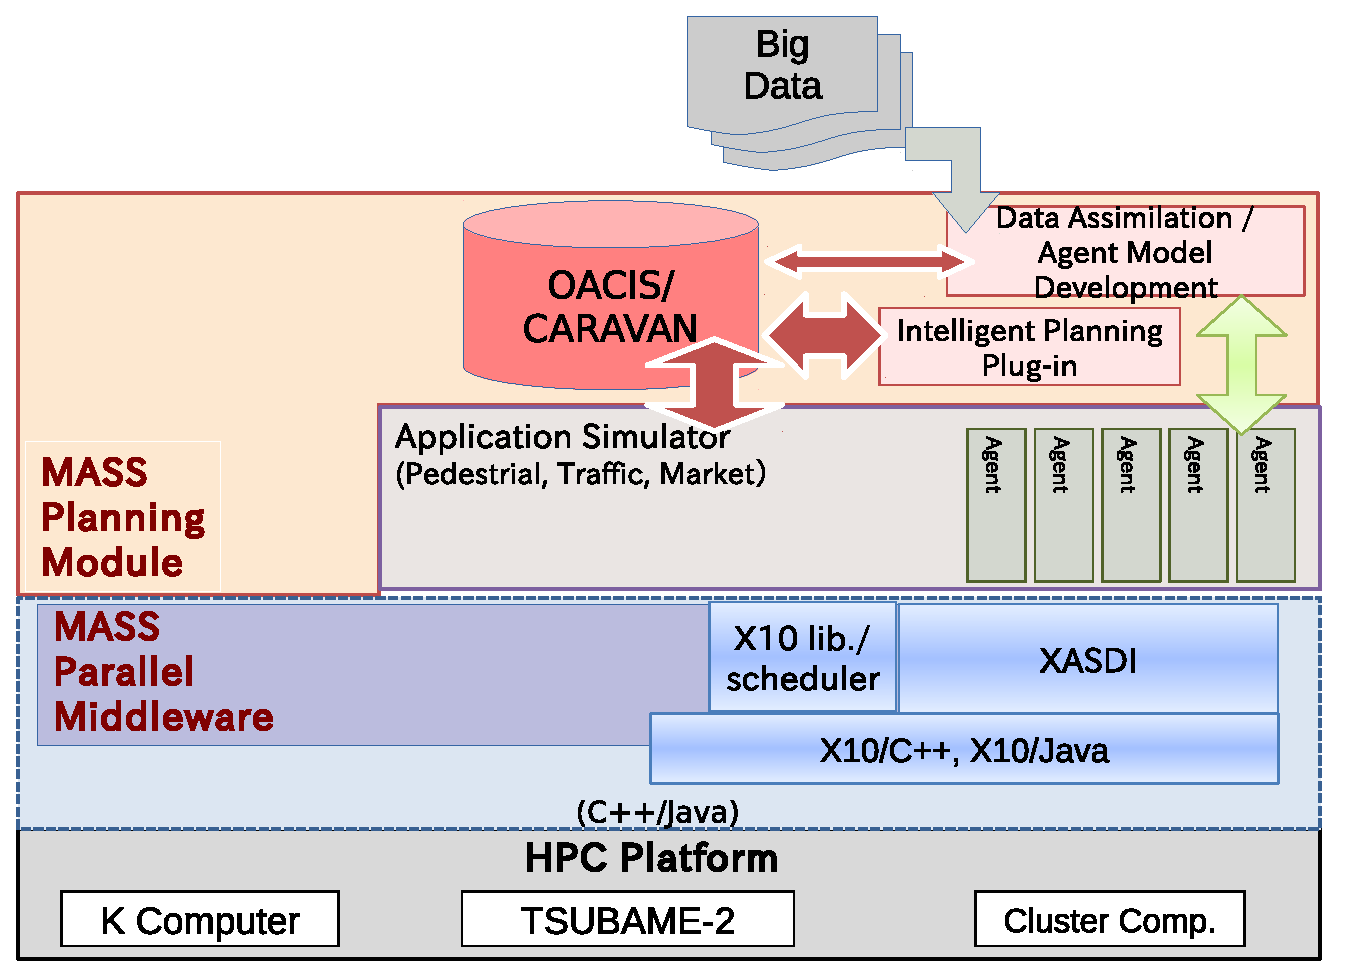
\includegraphics[width=.8\linewidth]{Figs.noda/figure-01.framework.eps}
  \caption{Cassia Framework}
  \label{fig:Figs.noda/figure-01.framework.eps}
\end{figure}
%%++++++++++++++++++++++++++++++++++++++++++++++++++++++++++++++++++++++


%%----------------------------------------------------------------------
\section{MASS Planning Module}
\label{s:MASS Planning Module}
%% - - - - - - - - - - - - - - - - - - - - - - - - - - - - - - - - - - -
(Murase, Ito)

OACIS (Organizing Assistant for Comprehensive and Interactive
Simulations) is a job management software for large-scale
simulations. It controls a large number of simulation jobs executed in
various remote servers, keeps these results in an organized way, and
manages the analyses on these results.

%%++++++++++++++++++++++++++++++++++++++++++++++++++++++++++++++++++++++
\begin{figure}
  \centering
  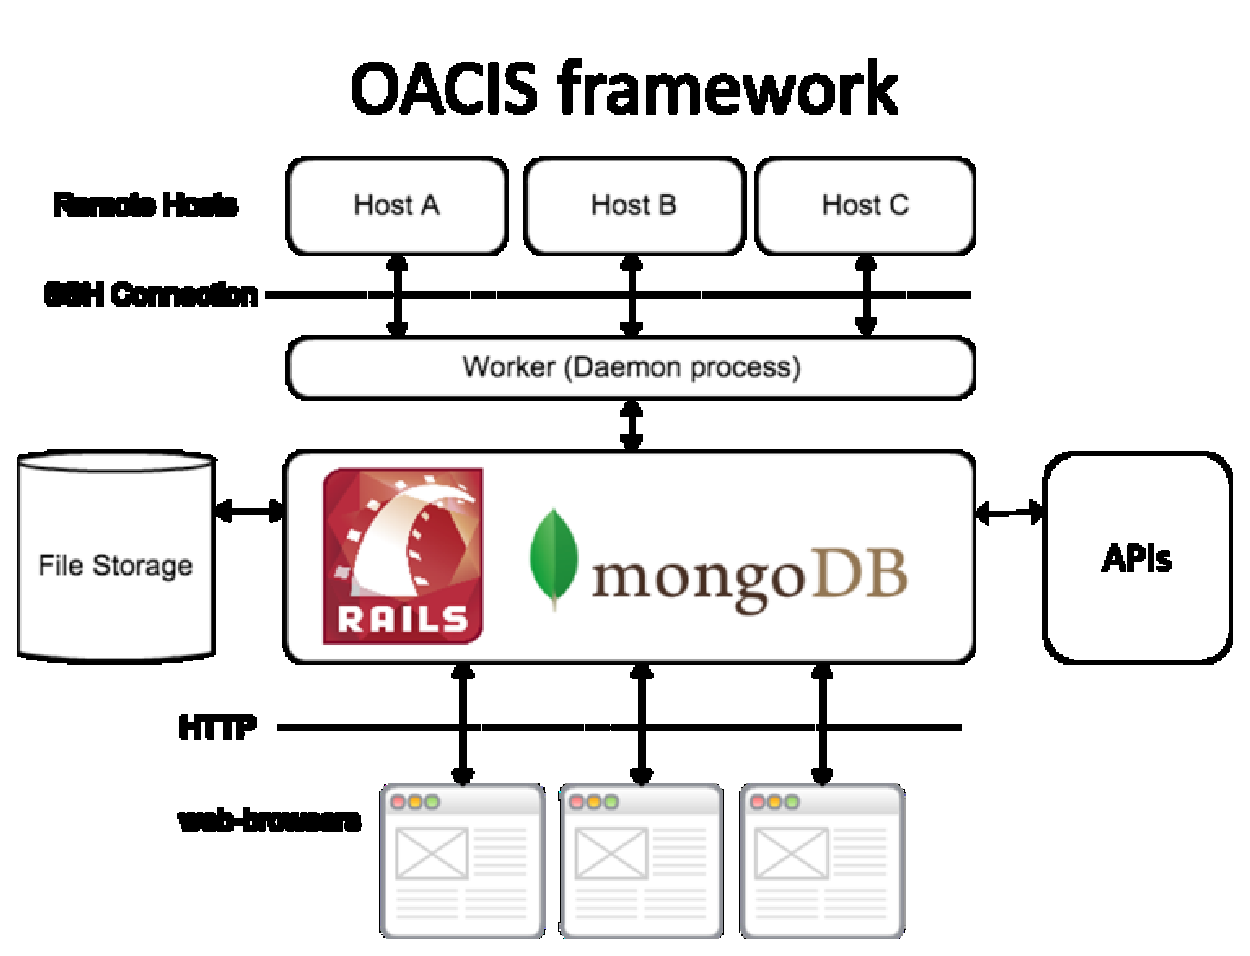
\includegraphics[width=.8\linewidth]{Figs.noda/figure-02.oacis.eps}
  \caption{OACIS}
  \label{fig:Figs.noda/figure-02.oacis.eps}
\end{figure}
%%++++++++++++++++++++++++++++++++++++++++++++++++++++++++++++++++++++++

CARAVAN provides more powerful scalability for exhaustive
simulation. These functionalities are especially beneficial for the
complex simulation models having many parameters for which a lot of
parameter searches are required.

%%++++++++++++++++++++++++++++++++++++++++++++++++++++++++++++++++++++++
\begin{figure}
  \centering
  
\includegraphics[width=.8\linewidth]{Figs.noda/figure-03.caravan.eps}
  \caption{CARAVAN}
  \label{fig:Figs.noda/figure-03.caravan.eps}
\end{figure}
%%++++++++++++++++++++++++++++++++++++++++++++++++++++++++++++++++++++++

%%----------------------------------------------------------------------
\section{MASS Parallel Middleware}
\label{s:MASS Parallel Middleware}
%% - - - - - - - - - - - - - - - - - - - - - - - - - - - - - - - - - - -


%%--------------------------------------------------
\subsection{X10 Extentions and Plham}
\label{ss:X10 Extentions and Plham}
%% - - - - - - - - - - - - - - - - - - - - - - - - -
(Kamada)

Plham is a platform for large-scale and high-frequency artificial
market simulation.  It consists of models of markets for each stocks
and three types of agents (high-freq. traders, short-term and
long-term traders).

In order to enhance parallelism of computation, we introduce
asynchronous computation in agents and communication between
agents/markets, and provide high-level library to program them.

%%++++++++++++++++++++++++++++++++++++++++++++++++++++++++++++++++++++++
\begin{figure}
  \centering
  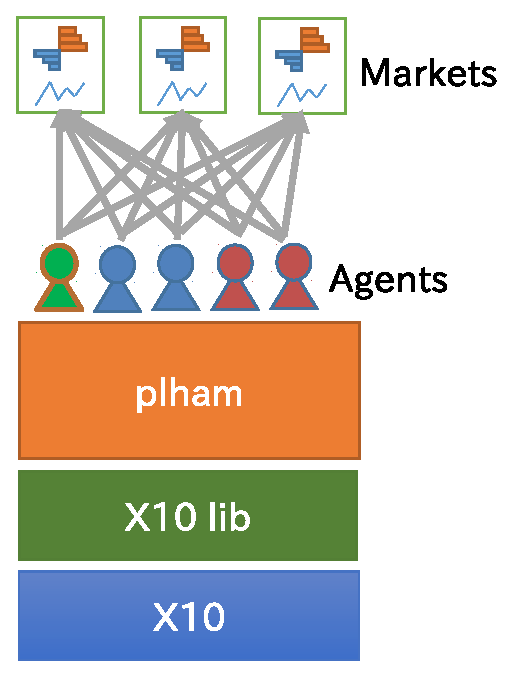
\includegraphics[width=.8\linewidth]{Figs.noda/figure-05.plham.eps}
  \caption{Plham}
  \label{fig:Figs.noda/figure-05.plham.eps}
\end{figure}
%%++++++++++++++++++++++++++++++++++++++++++++++++++++++++++++++++++++++

%%++++++++++++++++++++++++++++++++++++++++++++++++++++++++++++++++++++++
\begin{figure}
  \centering
  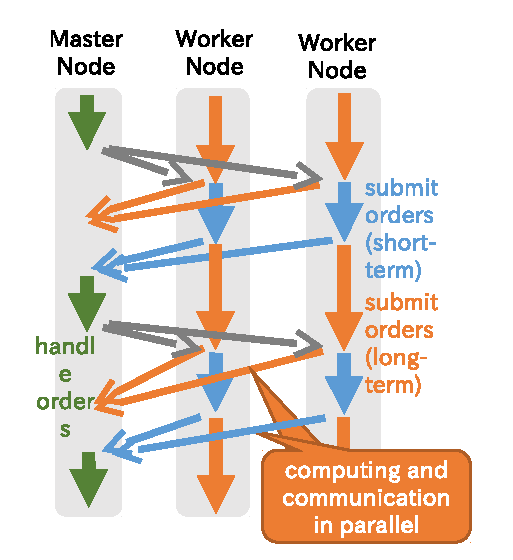
\includegraphics[width=.8\linewidth]{Figs.noda/figure-06.market_para.eps}
  \caption{Parallel Execution of Market Simulation}
  \label{fig:Figs.noda/figure-06.market_para.eps}
\end{figure}
%%++++++++++++++++++++++++++++++++++++++++++++++++++++++++++++++++++++++


%%--------------------------------------------------
\subsection{XASDI}
\label{ss:XASDI}
%% - - - - - - - - - - - - - - - - - - - - - - - - -
(Mizuta)

XASDI is the Large-scale agent-based social simulation framework with
billions of distributed agents that provides easy-to-use API bridge
with Java and X10-based runtime for high scalability. XASDI
environment executes various social simulations written in Java with
distributed agents and managers written in X10.

%%++++++++++++++++++++++++++++++++++++++++++++++++++++++++++++++++++++++
\begin{figure}
  \centering
  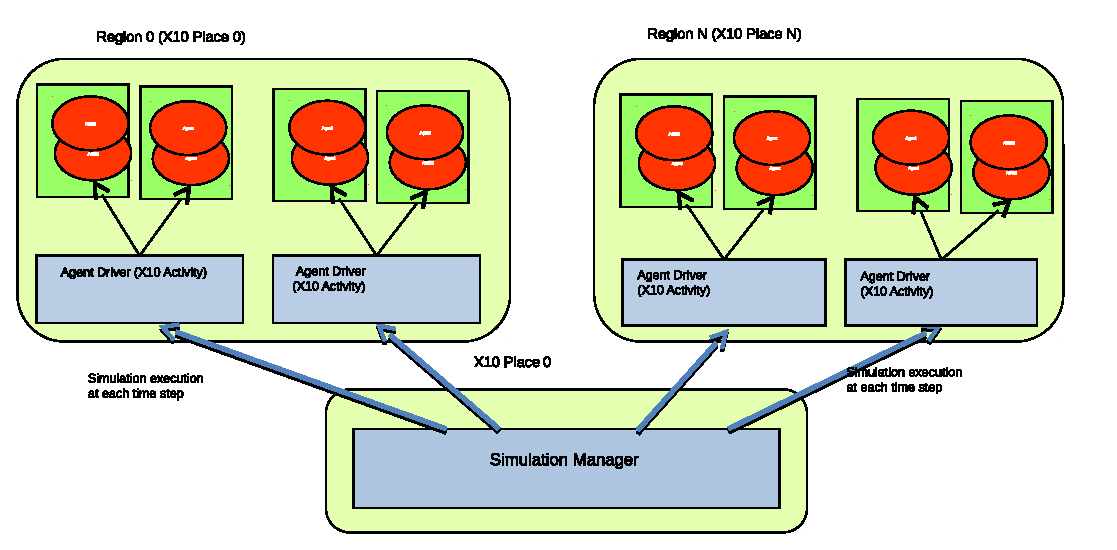
\includegraphics[width=.8\linewidth]{Figs.noda/figure-04.xasdi.eps}
  \caption{XASDI}
  \label{fig:Figs.noda/figure-04.xasdi.eps}
\end{figure}
%%++++++++++++++++++++++++++++++++++++++++++++++++++++++++++++++++++++++

%%----------------------------------------------------------------------
\section{Applications}
\label{s:Applications}
%% - - - - - - - - - - - - - - - - - - - - - - - - - - - - - - - - - - -

%%--------------------------------------------------
\subsection{Market Simulation}
\label{ss:Market Simulation}
%% - - - - - - - - - - - - - - - - - - - - - - - - -
(Izumi)

%%++++++++++++++++++++++++++++++++++++++++++++++++++++++++++++++++++++++
\begin{figure}
  \centering
  \includegraphics[width=.8\linewidth]{Figs.noda/figure-07.market_phase.eps}
  \caption{Phase Diagram of Market Simulation}
  \label{fig:Figs.noda/figure-07.market_phase.eps}
\end{figure}
%%++++++++++++++++++++++++++++++++++++++++++++++++++++++++++++++++++++++

%%--------------------------------------------------
\subsection{Pedestrian Simulation}
\label{ss:Pedestrian Simulation}
%% - - - - - - - - - - - - - - - - - - - - - - - - -
(Noda)

CASSIA Framework can illustrate a trade-off structure in planning of
evacuations from disasters.  Optimization in disaster responses is
serious requirements for local governments. But, such optimization
includes multiple objective functions.  So, the important issue is how
to understand trade-off structures of such multi-objective functions
over large number of policy options.

We apply our framework to evaluate evacuation plans, which have over
300 control parameters, to find out such trade-off.  We implement
NSGA-II algorithm to search optimal structures over large parameter
spaces, and utilize the performance of K-computers to speed-up the
process.

%%++++++++++++++++++++++++++++++++++++++++++++++++++++++++++++++++++++++
\begin{figure}
  \centering
  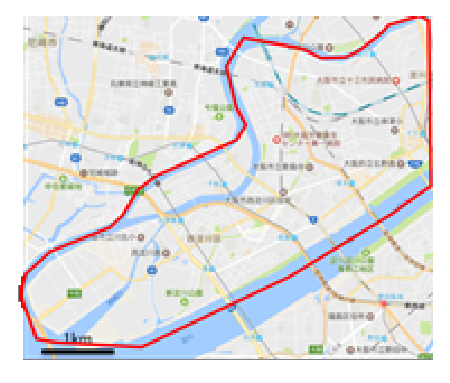
\includegraphics[width=.8\linewidth]{Figs.noda/figure-08.nishiyodogawa.eps}
  \caption{Nishiyodogawa Area used in Pedestrian Simulation}
  \label{fig:Figs.noda/figure-08.nishiyodogawa.eps}
\end{figure}
%%++++++++++++++++++++++++++++++++++++++++++++++++++++++++++++++++++++++

%%++++++++++++++++++++++++++++++++++++++++++++++++++++++++++++++++++++++
\begin{figure}
  \centering
  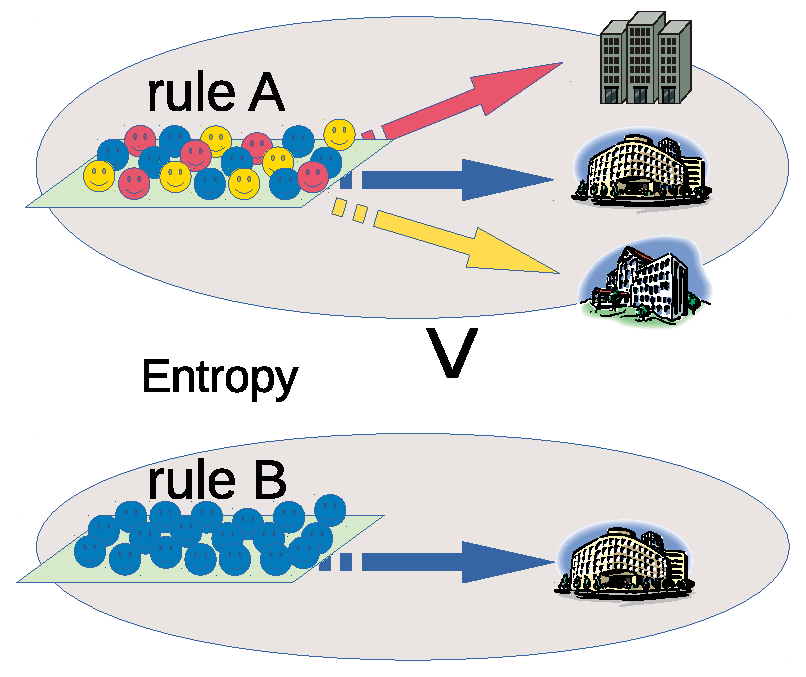
\includegraphics[width=.8\linewidth]{Figs.noda/figure-09.evac_rule.eps}
  \caption{Rule Entropy}
  \label{fig:Figs.noda/figure-09.evac_rule.eps}
\end{figure}
%%++++++++++++++++++++++++++++++++++++++++++++++++++++++++++++++++++++++

%%++++++++++++++++++++++++++++++++++++++++++++++++++++++++++++++++++++++
\begin{figure}
  \centering
  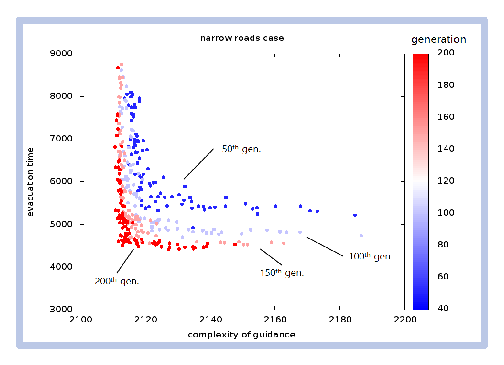
\includegraphics[width=.8\linewidth]{Figs.noda/figure-10.evac_narrow.eps}
  \caption{Result of Evacuation Simulation (narrow road)}
  \label{fig:Figs.noda/figure-10.evac_narrow.eps}
\end{figure}
%%++++++++++++++++++++++++++++++++++++++++++++++++++++++++++++++++++++++

%%++++++++++++++++++++++++++++++++++++++++++++++++++++++++++++++++++++++
\begin{figure}
  \centering
  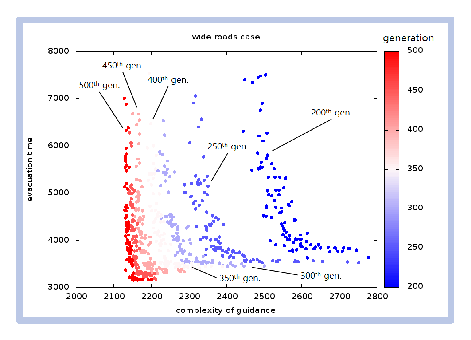
\includegraphics[width=.8\linewidth]{Figs.noda/figure-11.evac_wide.eps}
  \caption{Result of Evacuation Simulation (wide road)}
  \label{fig:Figs.noda/figure-11.evac_wide.eps}
\end{figure}
%%++++++++++++++++++++++++++++++++++++++++++++++++++++++++++++++++++++++


%%--------------------------------------------------
\subsection{Traffic Simulation}
\label{ss:Traffic Simulation}
%% - - - - - - - - - - - - - - - - - - - - - - - - -
(Hattori, Ito?)



